% !Mode:: "TeX:UTF-8"
% !TEX program  = xelatex
\documentclass[a4paper]{article}
\usepackage{amsmath}
\usepackage{amssymb}
\usepackage{ctex}
\usepackage{graphicx}
\usepackage[european]{circuitikz}
\usepackage{multirow}
\usepackage{enumitem}
\usepackage{geometry}
\usepackage{hyperref}
\geometry{a4paper, top=2cm, bottom=2cm, left=2cm, right=2cm}
\title{编程作业二报告}
\author{王凯灵 521030910356}
\date{2023年3月14日}
\begin{document}
	\section*{\Huge 编程作业二报告}
	\section*{\small 王凯灵 521030910356 2023年3月14日}
	本次作业要求对一个幅度为1，长度为10的矩形窗函数$x(t)$采样，平移，滤波等操作，并比较分析。
	
	(1)-(3): 使用$rectpuls$函数产生了窗函数，微调宽度确保了符合0和10处值为1的定义。在第三部分中，调试了特殊的滤波器初始参数使得效果比较明显。实际使用时应选择合适的参数。
	
	(4) 为方便表示，设采样频率$fs$是整数3， 即$t_s=\frac{1}{3}$，在实现中，从0到1000采样了3001处点作为无穷远的近似，所以令$N=3001$，原信号时域采样结果可以表示为
	\begin{equation}
	x[n] = \sum_{i=0}^{30}\delta(n-i)\text{，于是}
	X_1(\omega)=\sum_{n=-\infty}^{+\infty} x[n] e^{-j \omega n}=\sum_{n=0}^{30} e^{-j \omega n}=\frac{1-e^{-31 j \omega}}{1-e^{-j \omega}}\text{。}
	\end{equation}
	考虑到MATLAB中，fft函数实际上计算了给定信号的DFT，故给出DFT的表达式
	\begin{equation}
	X_1[k] = \sum_{n=0}^{30}x[n]e^{-\frac{j2\pi n k}{3001}}=\sum_{n=0}^{30} e^{-\frac{j2\pi n k}{3001}} = \frac{1-e^{-\frac{j 62\pi k}{3001}}}{1-e^{-\frac{j 2\pi k}{3001}}}\text{。三角函数没有指数形式优雅，此不给出。}
	\end{equation}
	将$x(t)$进行平移得到$x'(t)$，为作图统一，使用右移，即$x'(t)=x(t-\frac{t_s}{2})$。此时采样可以表示为
	\begin{equation}
		x'[n] = \sum_{i=1}^{30}\delta(n-i)\text{，实际上就是少了一个采样点。同理可得}X_2[k] = e^{- \frac{j 2\pi}{3001}}\frac{1-e^{-\frac{j 60\pi k}{3001}}}{1-e^{-\frac{j 2\pi k}{3001}}}
	\end{equation}
	这里的时移不影响幅频特性，会对相频特性造成影响。与(2)式相比，主要区别是分子指数上的分子变小，对于频谱的影响是零点出现的周期增加了。另由帕斯瓦尔定理，
	\begin{equation}
		\frac{1}{N}\sum_{n=0}^{N-1}|x[n]|^2=\frac{1}{N}\sum_{k=0}^{N-1}|X[k]|^2
	\end{equation}
	易知移动后的信号采样结果DFT频谱峰值会降低，与数值信号带入结果一致。
	
	将式(2)，(3)的图像画出并与第一二部分得到的频谱对比，可见是完全一样的，且与数学上的分析符合。

	使用一个滤波器$h(t)$对$x'(t)$滤波。滤波器参数在代码中明确给出，此处不进行表达式计算。
	\begin{equation}
		\text{易得}X(\omega) = \frac{2\sin(5\omega)}{\omega}e^{-j5\omega}\text{，采样在频域表示为}(X(\omega)\cdot H(\omega))*\left[\frac{2 \pi}{t_s} \sum_{k=0}^{+\infty} \delta\left(\omega-k \frac{2 \pi}{t_s}\right)\right]
	\end{equation}
	由于使用低通滤波器，高频分量受抑制，观察频谱图可以发现，大于0.7的频率分量明显减弱了。
	\newpage
	\section{附录：图像}
		\begin{figure}[h!]
			\begin{minipage}[t]{0.5\linewidth}
				\centering
				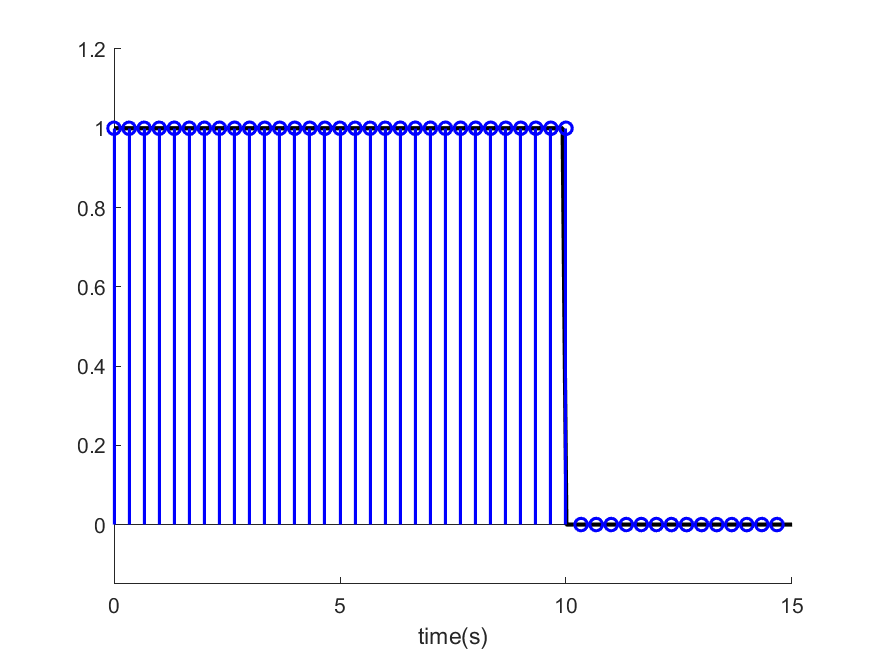
\includegraphics[width=0.9\textwidth]{../code/figures/p1}
				\caption{原信号时域采样}
			\end{minipage}
			\begin{minipage}[t]{0.5\linewidth}
				\centering
				
\includegraphics[width=0.9\textwidth]{../code/figures/p3}
				\caption{平移后时域采样}
			\end{minipage}
		\end{figure}
	
		\begin{figure}[h!]
			\begin{minipage}[t]{0.5\linewidth}
				\centering
				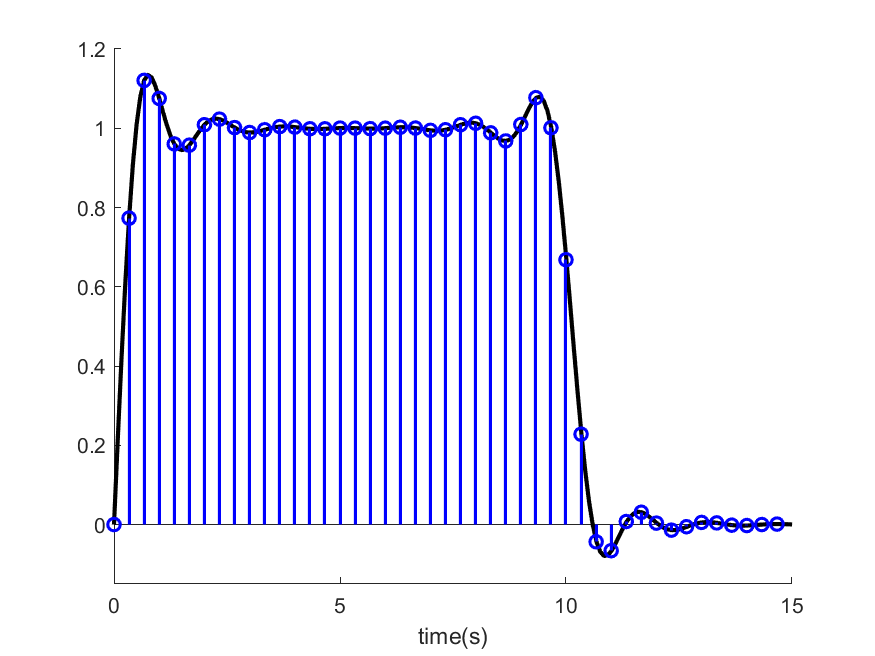
\includegraphics[width=0.9\textwidth]{../code/figures/p5}
				\caption{滤波后采样}
			\end{minipage}
			\begin{minipage}[t]{0.5\linewidth}
				\centering
				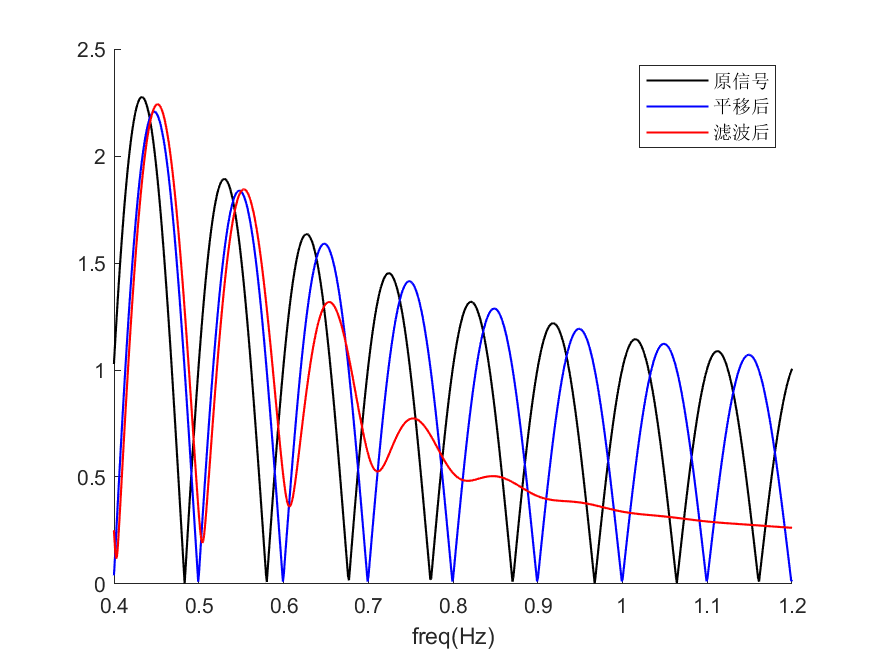
\includegraphics[width=0.9\textwidth]{../code/figures/p7}
				\caption{三种信号比较：截止频率处}
			\end{minipage}
		\end{figure}

		\begin{figure}[h!]
			\centering
			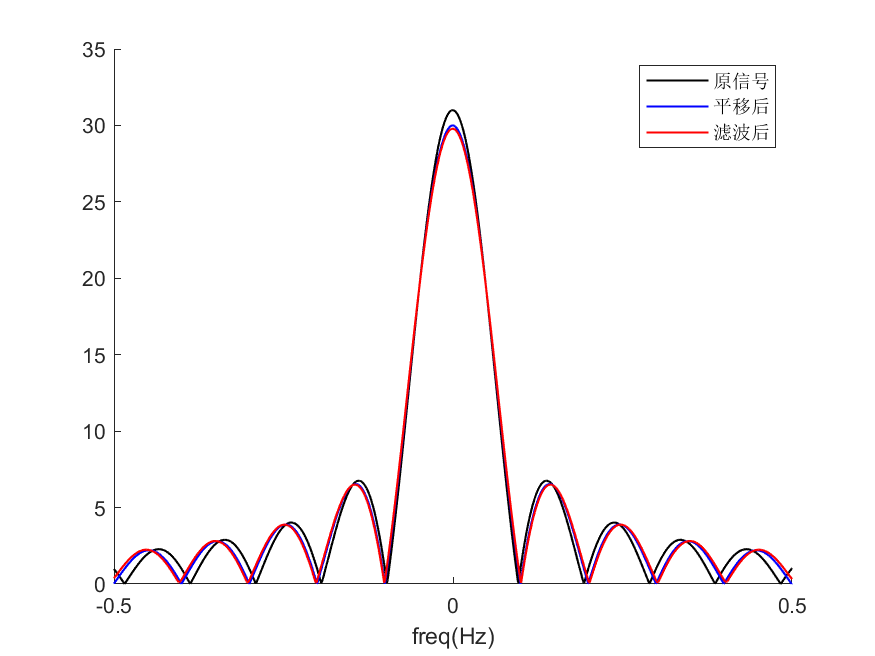
\includegraphics[width=0.75\textwidth]{../code/figures/p6}
			\caption{三种信号比较：原点附近}
		\end{figure}
	
		\begin{figure}[h!]
			\centering
			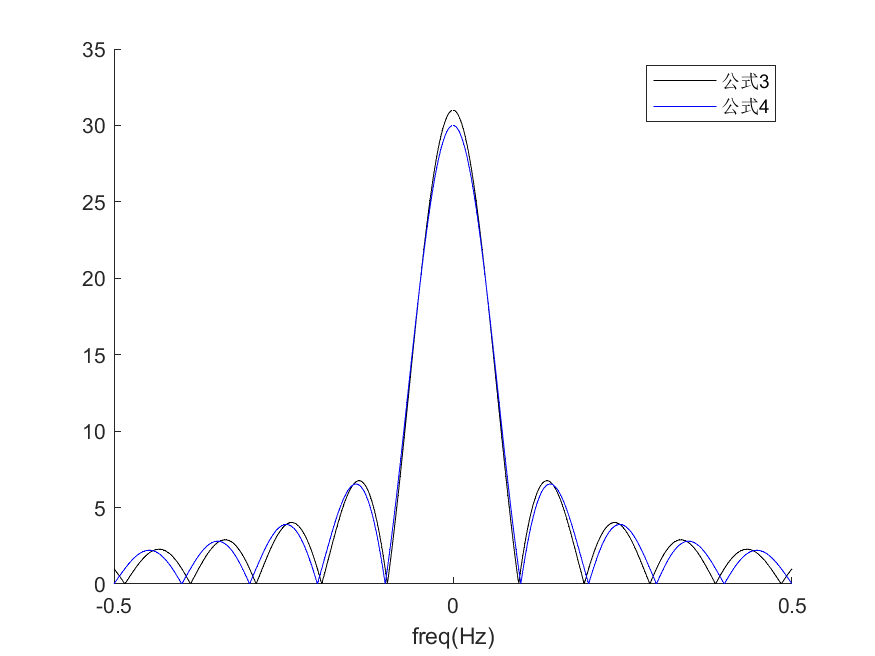
\includegraphics[width=0.75\textwidth]{../code/figures/p14}
			\caption{推导公式2，3函数图像}
		\end{figure}
\end{document}